% =============================================================================
% Title:        Reconstruction
% Author:       Nathaniel Thomas
% Affiliation:  Texas A&M University, Department of Nuclear Engineering
% Email:        nathaniel@tamu.edu
% Date Created: 3/7/2026
% Version:      1.0
%
% Description:
%   A .tex source file describing the reconstruction of the FLiNaK purifier.
%
% =============================================================================

\section{Reconstruction}
\label{sec: reconstruction}

% TODO: Incomplete

\begin{figure}[H]
  \centering
  \begin{subfigure}{0.49\textwidth}
    \centering
    \includegraphics[width=0.6\textwidth]{./assets/pictures/salt port
    flange before cleaning top.jpg}
    \caption{View of the top of the flange on the salt feed port
    before sandblasting. (01-23-2026)}
    \label{fig:salt port
    flange before cleaning top}
  \end{subfigure}
  \hfill
  \begin{subfigure}{0.49\textwidth}
    \centering
    \includegraphics[width=0.6\textwidth]{./assets/pictures/salt port
    flange before cleaning bottom.jpg}
    \caption{View of the bottom of the flange on the salt feed port
    before sandblasting. (01-23-2026)}
    \label{fig:salt port
    flange before cleaning bottom}
  \end{subfigure}
\end{figure}

\begin{figure}[H]
  \centering
  \begin{subfigure}{0.49\textwidth}
    \centering
    \includegraphics[width=0.6\textwidth]{./assets/pictures/salt port
    flange after cleaning top.jpg}
    \caption{View of the top of the flange on the salt feed port
    after sandblasting. (01-23-2026)}
    \label{fig:salt port
    flange after cleaning top}
  \end{subfigure}
  \hfill
  \begin{subfigure}{0.49\textwidth}
    \centering
    \includegraphics[width=0.6\textwidth]{./assets/pictures/salt port
    flange after cleaning bottom.jpg}
    \caption{View of the bottom of the flange on the salt feed port
    after sandblasting. (01-23-2026)}
    \label{fig:salt port
    flange after cleaning bottom}
  \end{subfigure}
\end{figure}

\begin{figure}[H]
  \centering
  \includegraphics[width=0.6\textwidth]{./assets/pictures/cleaned
  transfer tank lid top.jpg}
  \caption{View of the top of the transfer tank lid after
  wirebrushing. (01-23-2026)}
  \label{fig:cleaned transfer tank lid top}
\end{figure}

\begin{figure}[H]
  \centering
  \includegraphics[width=0.6\textwidth]{./assets/pictures/cleaned
  transfer tank lid bottom.jpg}
  \caption{View of the bottom of the transfer tank lid after
  wirebrushing. (01-23-2026)}
  \label{fig:cleaned transfer tank lid bottom}
\end{figure}

\begin{figure}[H]
  \centering
  \includegraphics[width=0.6\textwidth]{./assets/pictures/sandblasted
  transfer tank lid top.jpg}
  \caption{View of the top of the transfer tank lid after
  sandblasting. (01-23-2026)}
  \label{fig:sandblasted transfer tank lid top}
\end{figure}

\begin{figure}[H]
  \centering
  \includegraphics[width=0.6\textwidth]{./assets/pictures/sandblasted
  transfer tank lid bottom.jpg}
  \caption{View of the bottom of the transfer tank lid after
  sandblasting. (01-23-2026)}
  \label{fig: sandblasted transfer tank lid bottom}
\end{figure}

\begin{figure}[H]
  \centering
  \includegraphics[width=0.6\textwidth]{./assets/pictures/transfer
  tank comparison of before and after sandblasting.jpg}
  \caption{Side-by-side view of the transfer tank body before cleaning and the
  transfer tank lid after cleaning. (01-23-2026)}
  \label{fig: transfer tank comparison of before and after sandblasting}
\end{figure}

\begin{figure}[H]
  \centering
  \includegraphics[width=0.6\textwidth]{./assets/pictures/transfer
    tube sandblasted
  reducer.jpg}
  \caption{View of the sandblasted 3/4" to 1/2" Swageok reducer that
    coupled the salt transfer dip tube to the reaction chamber lid. Note
  the pitting corrosion caused by a brief exposure to FLiNaK. (01-23-2026)}
  \label{fig: transfer tube sandblasted reducer}
\end{figure}

\begin{figure}[H]
  \centering
  \includegraphics[width=0.6\textwidth]{./assets/pictures/transfer
    tube sandblasted
  reducer inside.jpg}
  \caption{View of the inside of the sandblasted 3/4" to 1/2" Swageok
    reducer that
  coupled the salt transfer dip tube to the reaction chamber lid. (01-23-2026)}
  \label{fig: transfer tube sandblasted reducer inside}
\end{figure}

\begin{figure}[H]
  \centering
  \includegraphics[width=0.6\textwidth]{./assets/pictures/cleaned
  reaction chamber lid top.jpg}
  \caption{View of the top of the reaction chamber lid after
  sandblasting. (01-23-2026)}
  \label{fig: cleaned reaction chamber lid top}
\end{figure}

\begin{figure}[H]
  \centering
  \includegraphics[width=0.6\textwidth]{./assets/pictures/cleaned
  reaction chamber lid bottom.jpg}
  \caption{View of the bottom of the reaction chamber lid after
  sandblasting. (01-23-2026)}
  \label{fig: cleaned reaction chamber lid bottom}
\end{figure}

\begin{figure}[H]
  \centering
  \includegraphics[width=0.6\textwidth]{./assets/pictures/cleaned
  transfer tank inside.jpg}
  \caption{Sandblasted transfer tank inside. (01-23-2026)}
  \label{fig: cleaned transfer tank inside}
\end{figure}

\begin{figure}[H]
  \centering
  \includegraphics[width=0.6\textwidth]{./assets/pictures/cleaned
  transfer tank bottom.jpg}
  \caption{Sandblasted transfer tank bottom (01-23-2026)}
  \label{fig: cleaned transfer tank bottom}
\end{figure}

\begin{figure}[H]
  \centering
  \includegraphics[width=0.6\textwidth]{./assets/pictures/thinned lid
  surrounding tube.jpg}
  \caption{A view of the underside of the transfer tank lid being milled
    out to reduce the thermal mass of the salt transfer tube entry point.
    This minimizes the heat removed from salt when entering the transfer tank.
    This thickness of the transfer tank at this point is about 5/16".
  (01-23-2026)}
  \label{fig: thinned lid surrounding tube}
\end{figure}

\begin{figure}[H]
  \centering
  \includegraphics[width=0.6\textwidth]{./assets/pictures/transfer
  tank new tube before welding.jpg}
  \caption{View of the new transfer tube in place before welding and
  cutting to length. (01-27-2026)}
  \label{fig: transfer tank new tube before welding}
\end{figure}

\begin{figure}[H]
  \centering
  \includegraphics[width=0.6\textwidth]{./assets/pictures/thinned lid
  with new tube.jpg}
  \caption{View of the underside of the transfer tank with the
    thinned lid portion and
  the new transfer tube in place, before welding. (01-27-2026)}
  \label{fig: thinned lid with new tube}
\end{figure}

\begin{figure}[H]
  \centering
  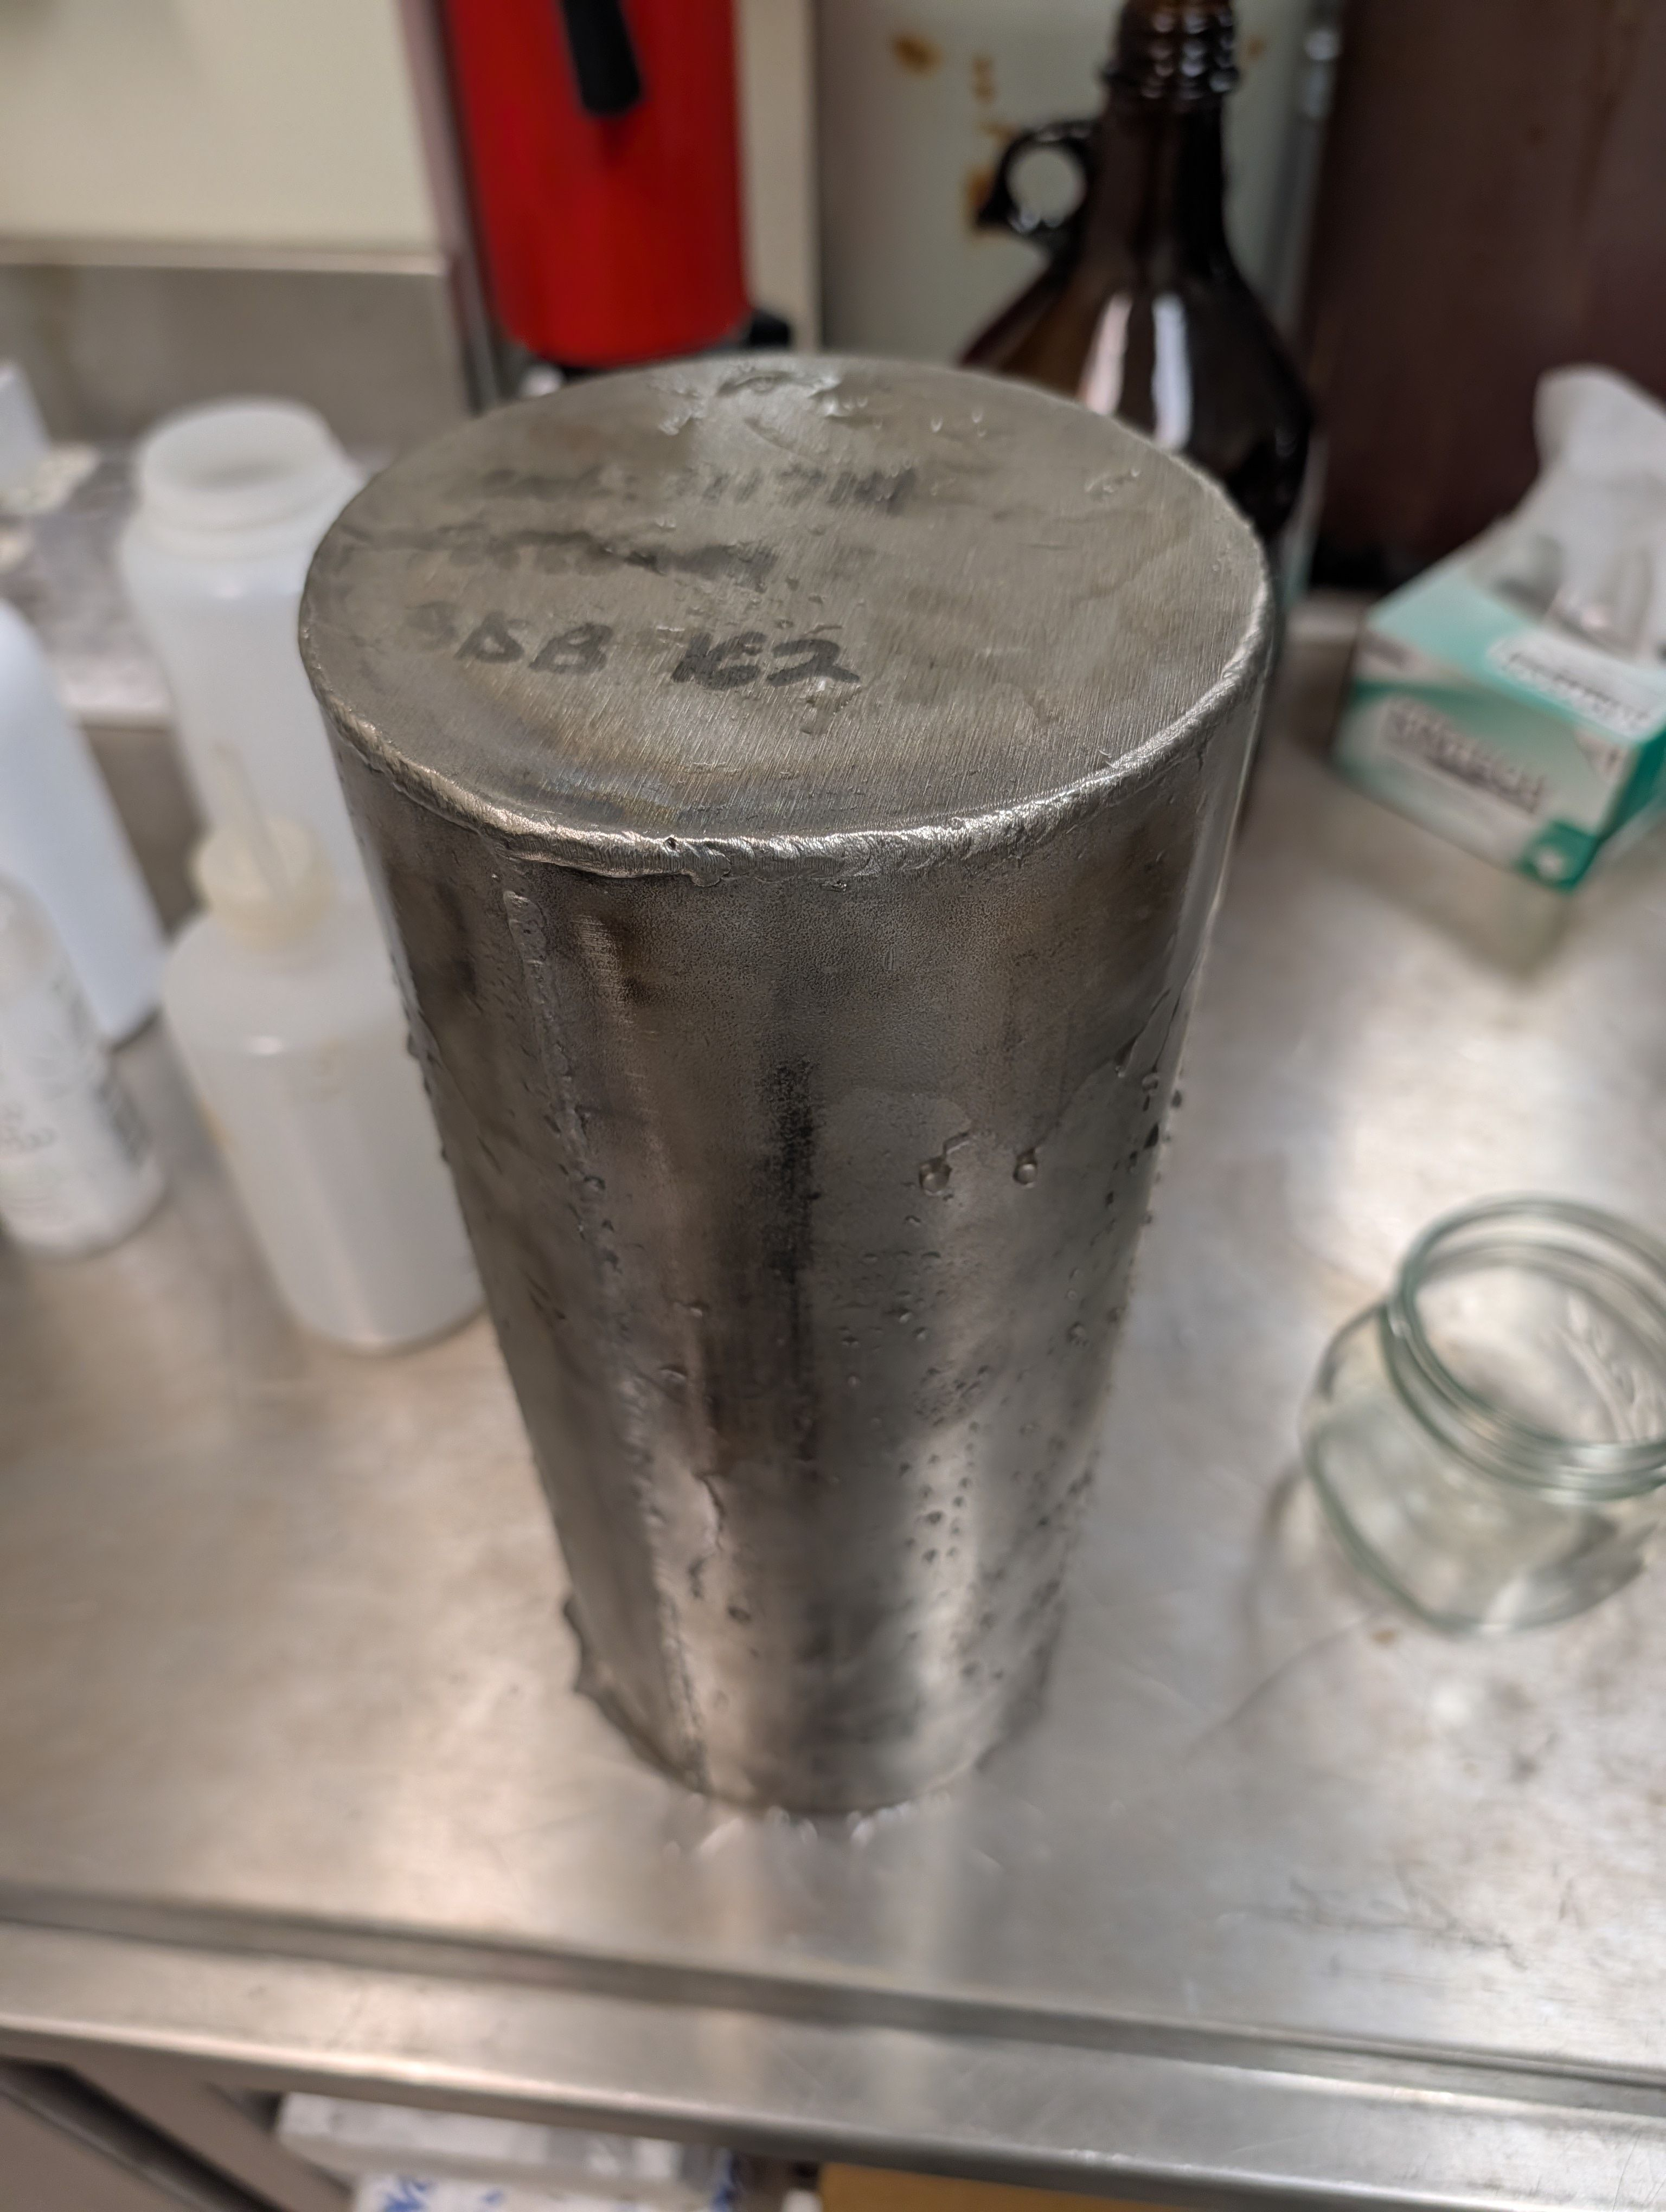
\includegraphics[width=0.6\textwidth]{./assets/pictures/ni liner washed.jpg}
  \caption{View of the new Ni liner constructed by Brazos Industries following
    washing with tap water.
  (02-28-2026)}
  \label{fig: new ni liner washed}
\end{figure}

\begin{figure}[H]
  \centering
  \includegraphics[width=0.6\textwidth]{./assets/pictures/ni liner
  washed inside.jpg}
  \caption{View of the inside of the new Ni liner constructed by
    Brazos Industries following
    washing with tap water.
  (02-28-2026)}
  \label{fig: new ni liner washed inside}
\end{figure}

\begin{figure}[H]
  \centering
  \includegraphics[width=0.6\textwidth]{./assets/pictures/ni liner
  washed rightside up.jpg}
  \caption{Alternate view of the new Ni liner constructed by
    Brazos Industries following
  washing with tap water. Note the weld seam. (02-28-2026)}
  \label{fig: new ni liner washed rightside up}
\end{figure}

\begin{figure}[H]
  \centering
  \includegraphics[width=0.6\textwidth]{./assets/pictures/ni liner
  bottom weld seam.jpg}
  \caption{Bottom weld seam of the new Ni liner. (02-28-2026)}
  \label{fig: ni liner bottom weld seam}
\end{figure}

\begin{figure}[H]
  \centering
  \includegraphics[width=0.6\textwidth]{./assets/pictures/finished
  and welded transfer tank lid.jpg}
  \caption{View of the bottom of the transfer tank lid welded and finished by
  Brazows Industries (02-28-2026)}
  \label{fig: finished and welded transfer tank lid}
\end{figure}

\begin{figure}[H]
  \centering
  \includegraphics[width=0.6\textwidth]{./assets/pictures/finished
  and welded transfer tank lid top.jpg}
  \caption{Top view of the bottom of the transfer tank lid welded and
    finished by
  Brazows Industries (02-28-2026)}
  \label{fig: finished and welded transfer tank lid top}
\end{figure}

\begin{figure}[H]
  \centering
  \includegraphics[width=0.6\textwidth]{./assets/pictures/reaction
  chamber lid washed bottom.jpg}
  \caption{Reaction chamber lid washed bottom. (02-28-2026)}
  \label{fig: reaction chamber lid washed bottom}
\end{figure}

\begin{figure}[H]
  \centering
  \includegraphics[width=0.6\textwidth]{./assets/pictures/reaction
  chamber lid washed top.jpg}
  \caption{Reaction chamber lid washed top. (02-28-2026)}
  \label{fig: reaction chamber lid washed top}
\end{figure}

\begin{figure}[H]
  \centering
  \includegraphics[width=0.6\textwidth]{./assets/pictures/reaction
  chamber base inside.jpg}
  \caption{A view of the reaction chamber inside wall. Note the
    corrosion still present.
    Due to the presence of a liner, totally removing the corrosion is
    not necessary. Also note the extensive corrosion around the weld
    seam on the bottom
  of the chamber. (02-28-2026)}
  \label{fig: reaction chamber base inside}
\end{figure}

\begin{figure}[H]
  \centering
  \includegraphics[width=0.6\textwidth]{./assets/pictures/transfer
  tank assembled and vacuumed.jpg}
  \caption{The transfer tank assembled and connected to a vacuum pump. Note only
    every other bolt hole is used, and Ni-graphite anti-sieze is used
    on the bolts. In addition,galvanized steel bolts were used.
    Vacuum came down to 20 mTorr.
    Anti-sieze:
    \href{https://www.mcmaster.com/1288K13/}{https://www.mcmaster.com/1288K13/}
    (03-01-2026)
  }
  \label{fig: transfer tank assembled and vacuumed}
\end{figure}

\begin{figure}[H]
  \centering
  \includegraphics[width=0.6\textwidth]{./assets/pictures/assembled transfer
  tank close up.jpg}
  \caption{Close-up view of the assembled transfer tank. Note the
    galvanized steel bolts and alignment
    of the helium leak-testing grooves. (03-01-2026)
  }
  \label{fig: assembled transfer tank close up}
\end{figure}

\begin{figure}[H]
  \centering
  \includegraphics[width=0.6\textwidth]{./assets/pictures/reaction
  chamber and liner}
  \caption{View of the reaction chamber and liner prior to assembly.
    (03-01-2026)
  }
  \label{fig: reaction chamber and liner}
\end{figure}

\begin{figure}[H]
  \centering
  \includegraphics[width=0.6\textwidth]{./assets/pictures/new dip
  tube bottom.jpg}
  \caption{New dip tube bottom with grooves cut to facilitate salt transfer.
    (03-01-2026)
  }
  \label{fig: new dip tube bottom}
\end{figure}

\begin{figure}[H]
  \centering
  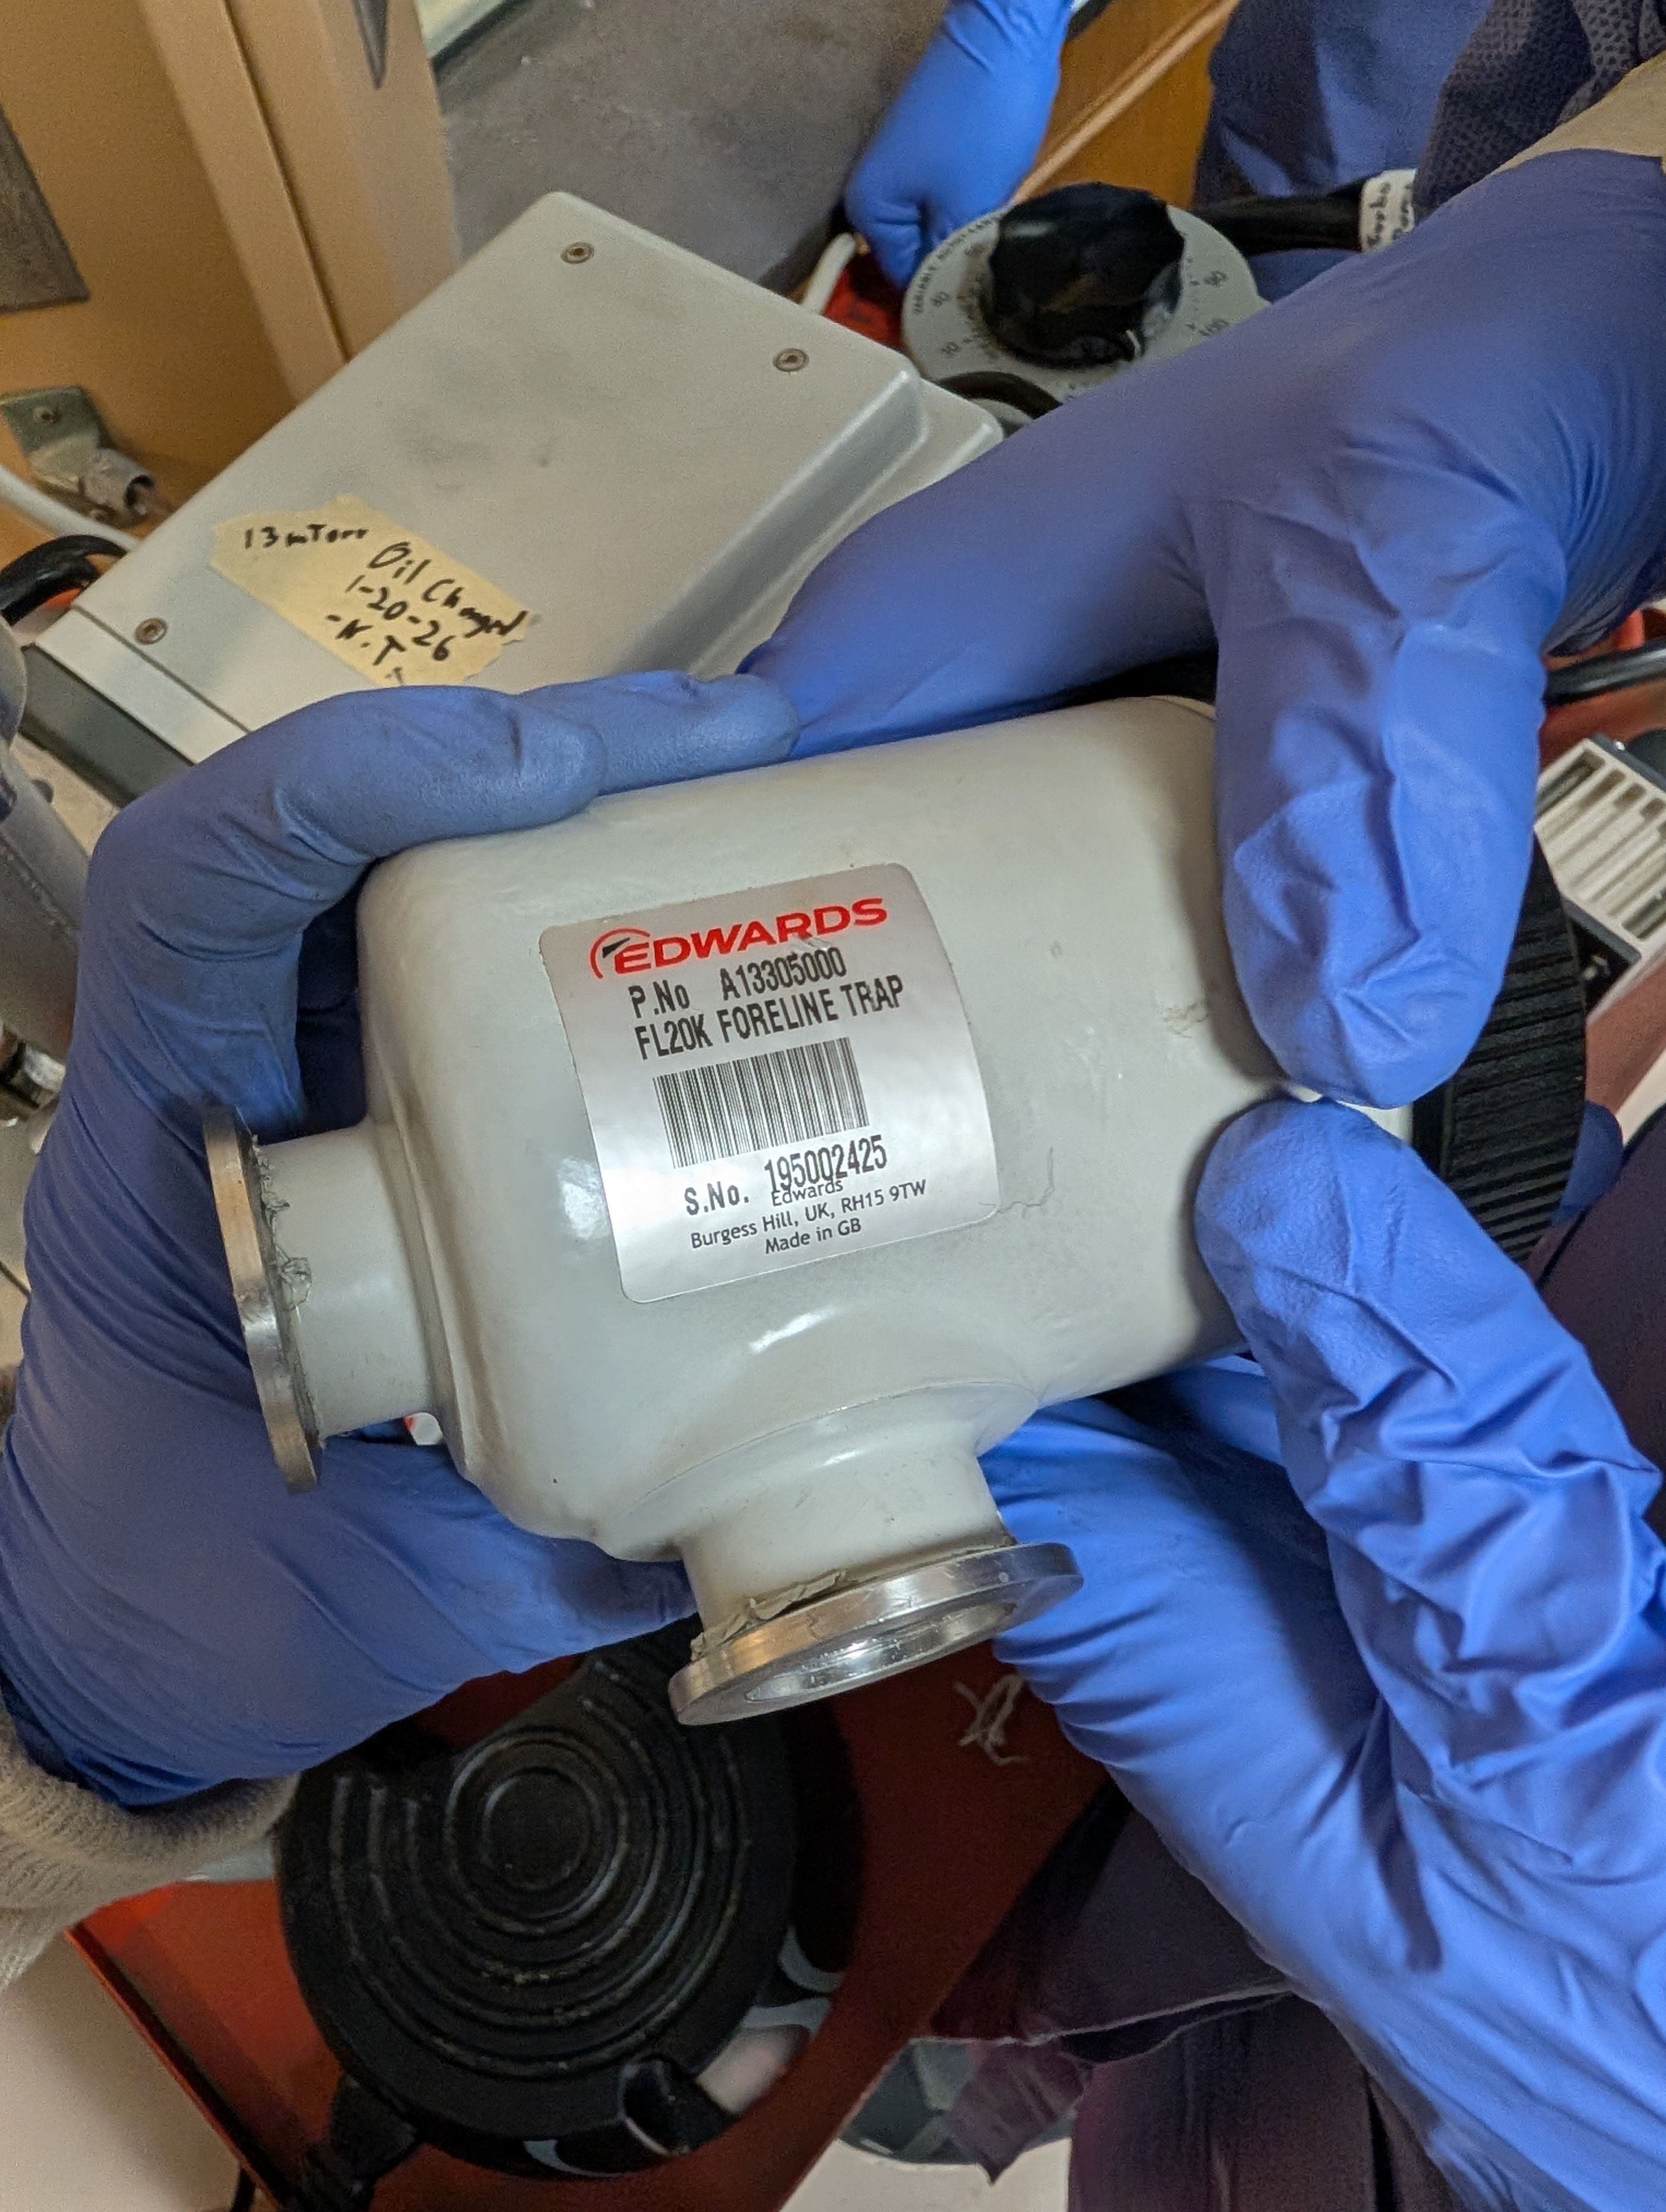
\includegraphics[width=0.6\textwidth]{./assets/pictures/new foreline trap.jpg}
  \caption{New foreline trap for the vacuum pump to protect
    the pump from corrosive vapors, and trap oil from entering the
    system. (03-02-2026)
  }
  \label{fig: new foreline trap}
\end{figure}

\begin{figure}[H]
  \centering
  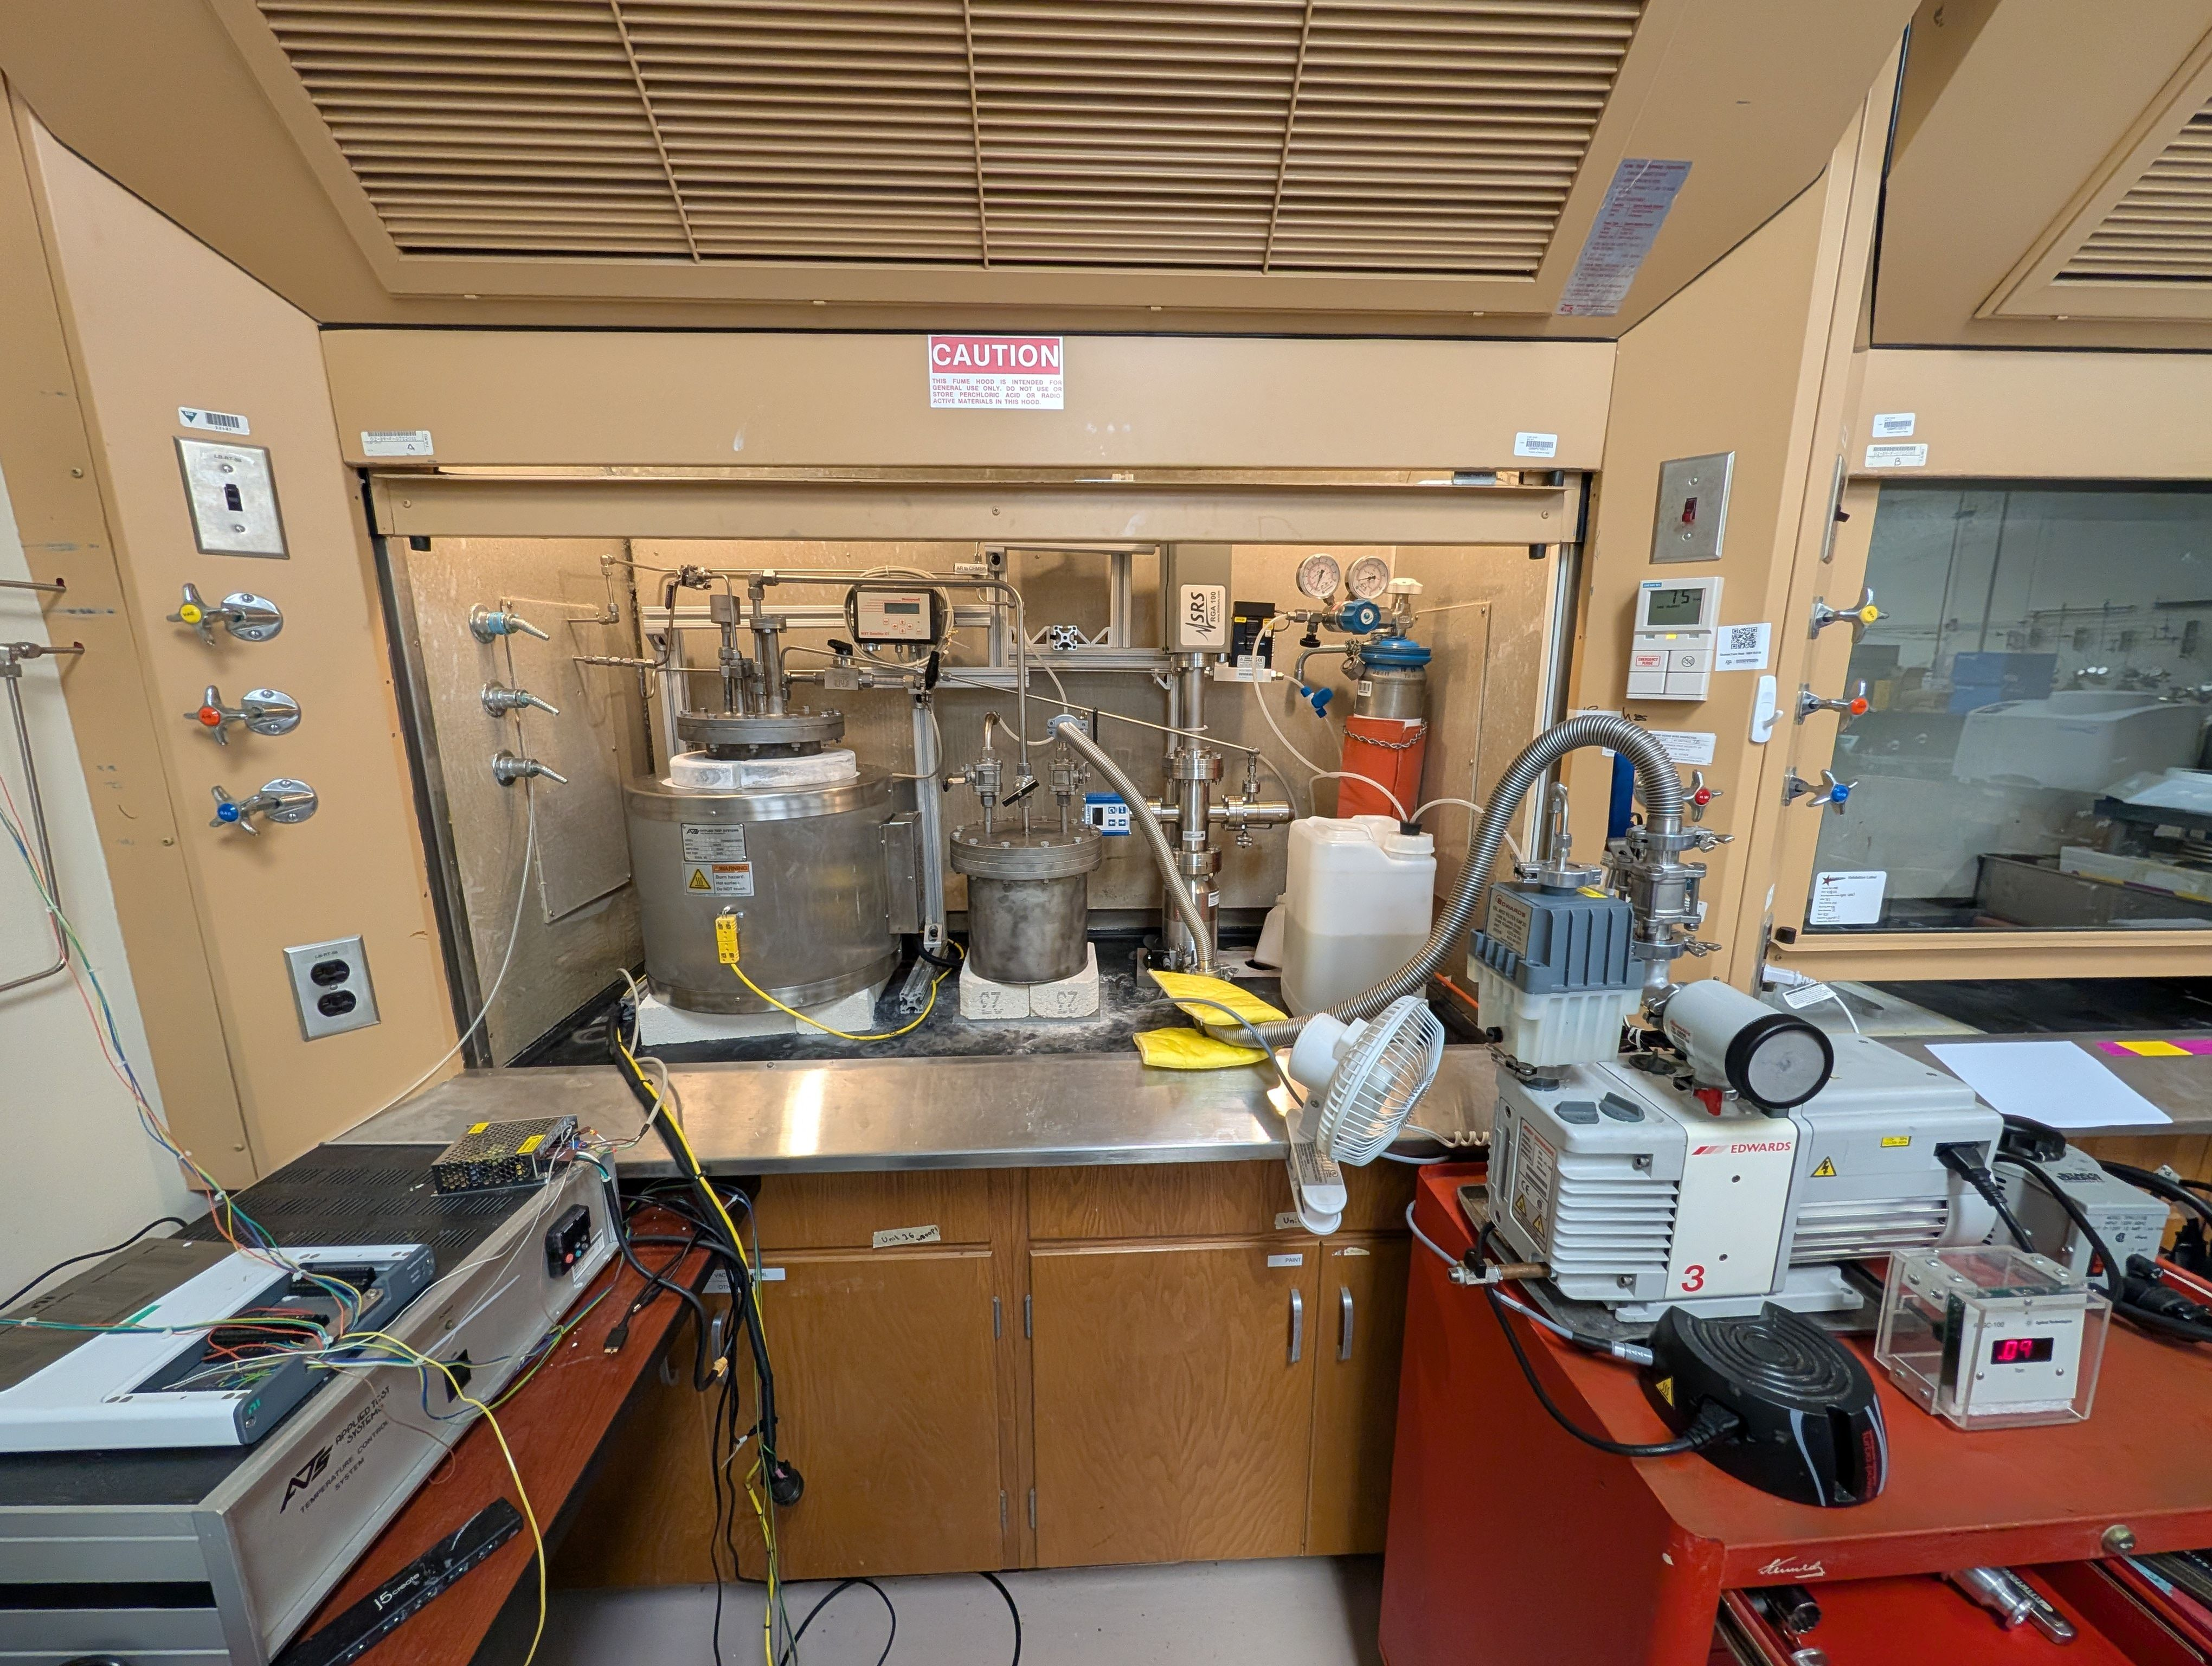
\includegraphics[width=0.6\textwidth]{./assets/pictures/system assembled.jpg}
  \caption{View of the newly assembled system. A 316L stainless steel pipe is
    used as the transfer line, as well as a 316L high temperature
    needle valve from Swagelok. Not ideal, but the C276 alternatives
    are expensive and have a long lead time. Short exposure to salt
    at temperature
    during transfer should have minimal corrosion. (03-03-2026)
  }
  \label{fig: system assembled}
\end{figure}

\begin{figure}[H]
  \centering
  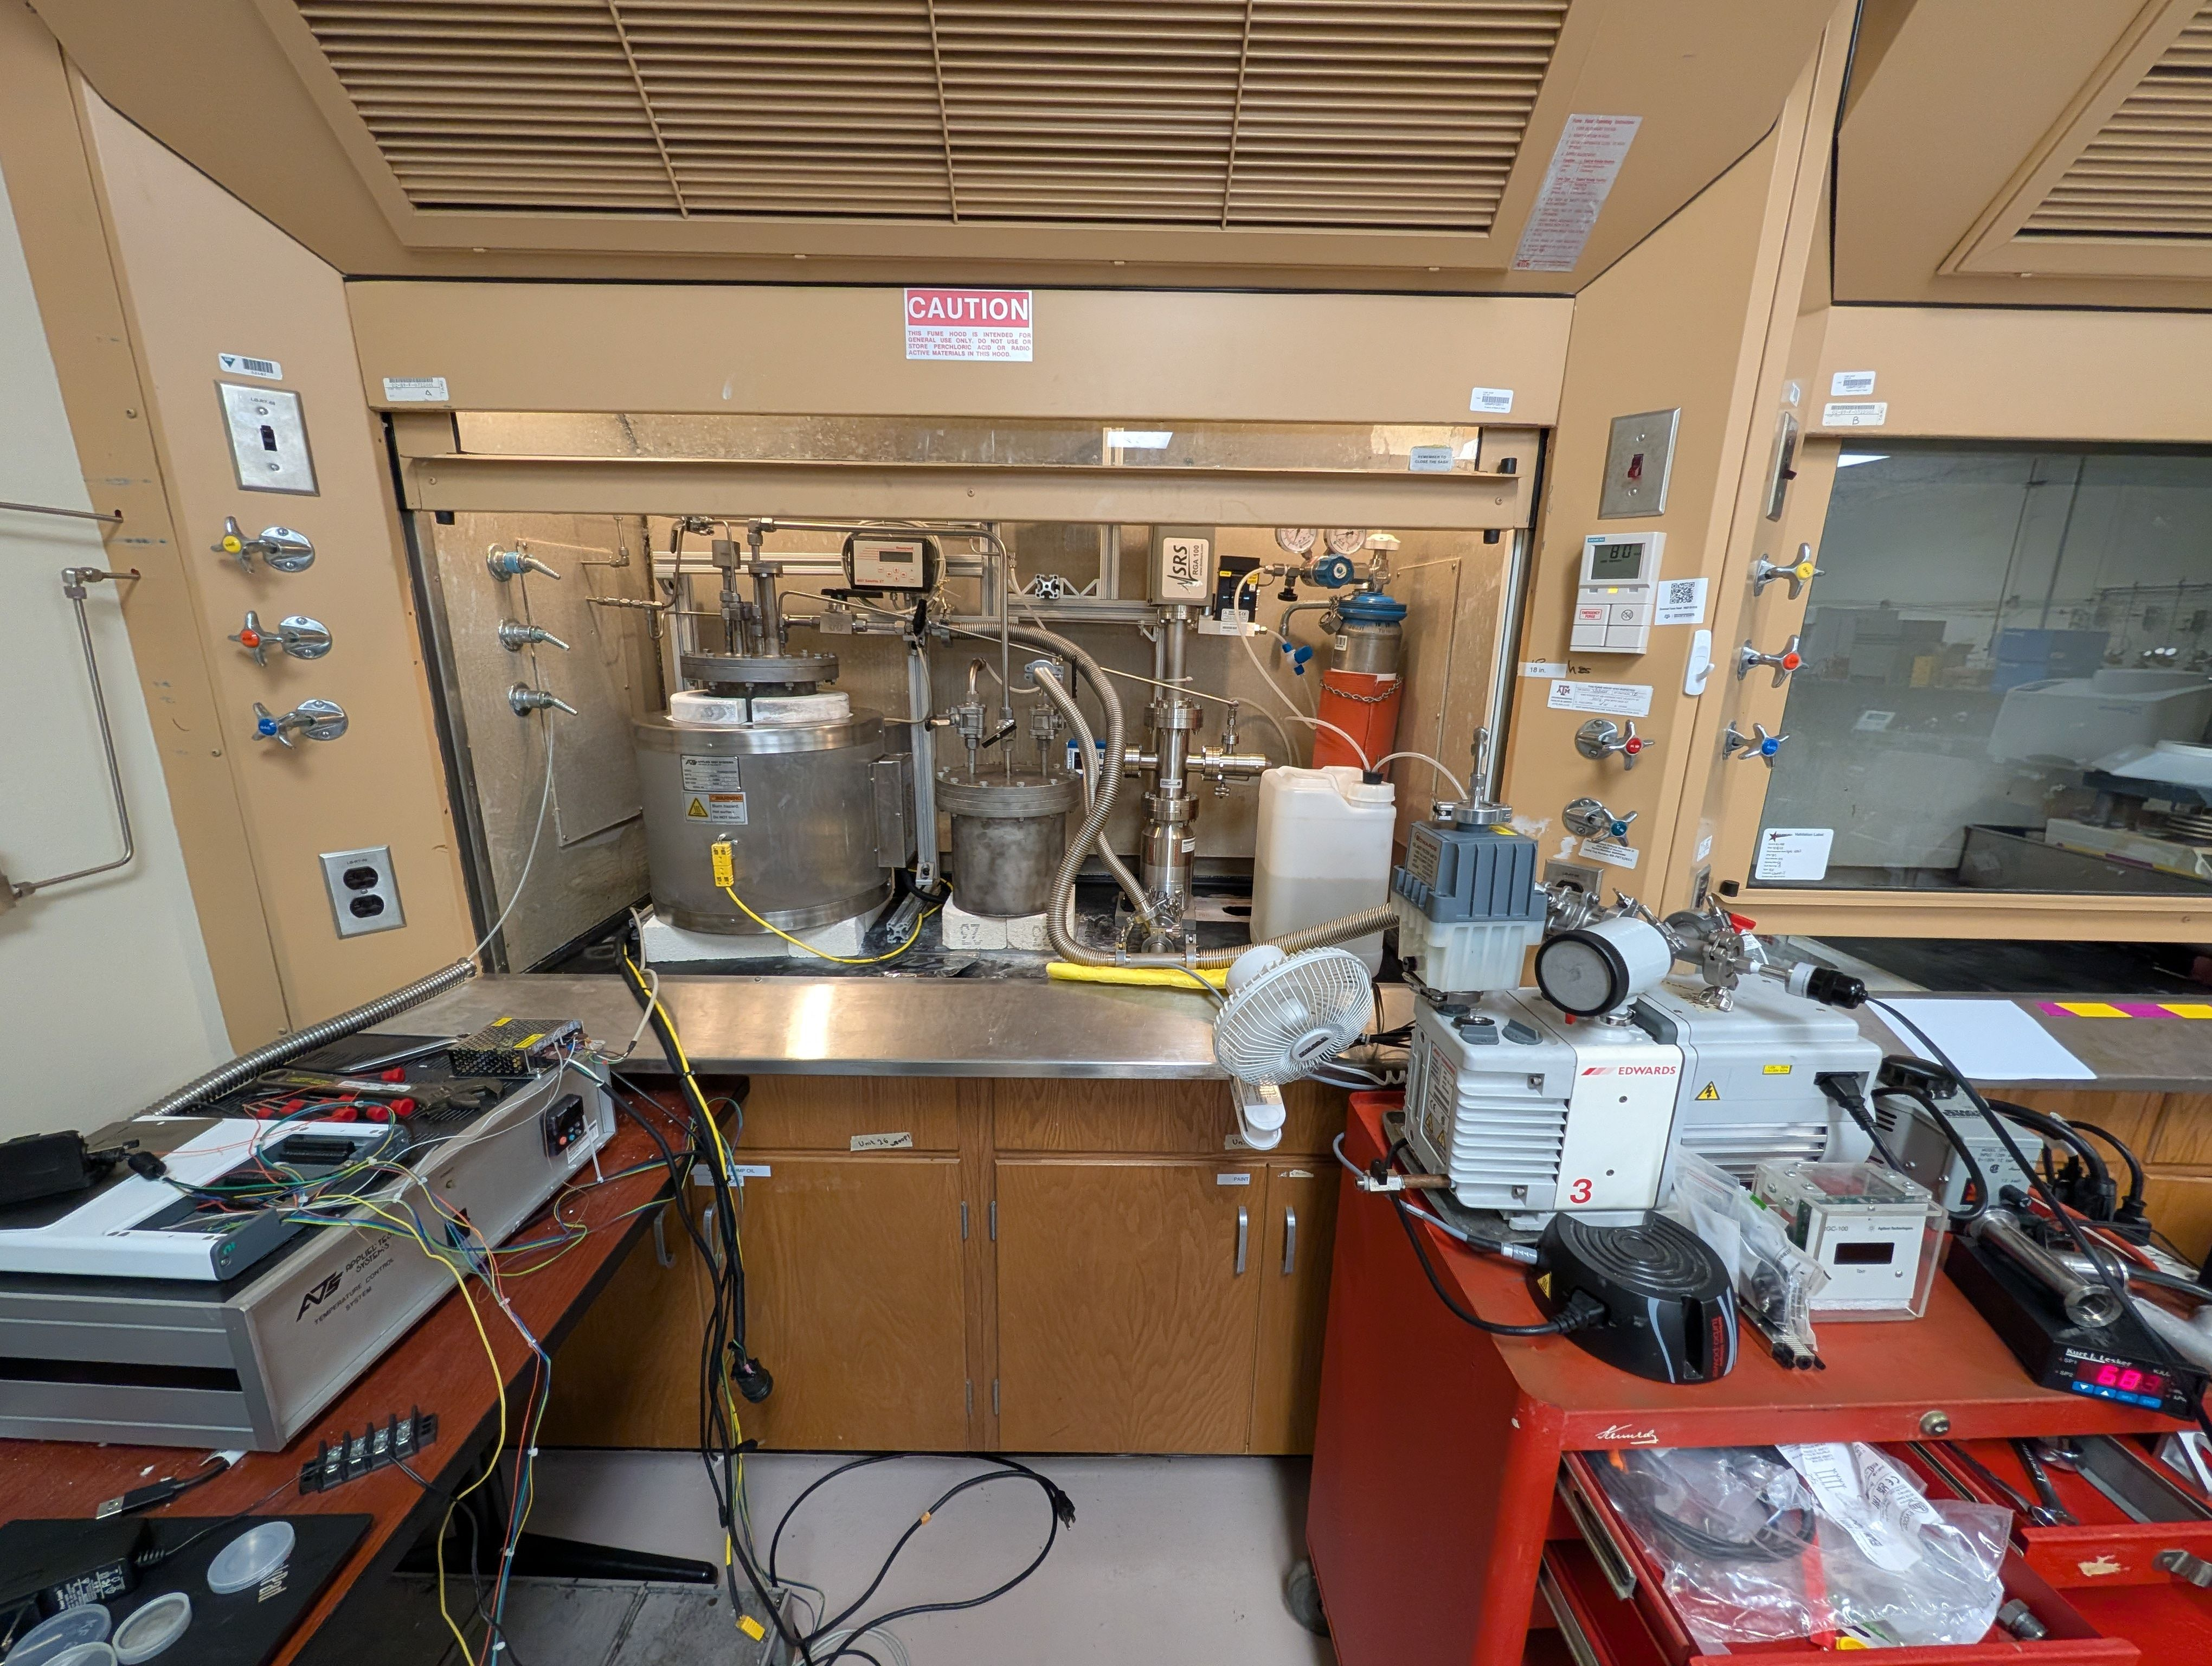
\includegraphics[width=0.6\textwidth]{./assets/pictures/new vacuum ducts.jpg}
  \caption{View of the assembled system with new vacuum ducts to
    enable purge/evacuation
    cycles to be performed on the reaction chamber without needing to
    switch vacuum
    lines. (03-03-2026)
  }
  \label{fig: new vacuum ducts}
\end{figure}

Notes on cleaning and assembly of transfer tank:
\begin{enumerate}
  \item Cleaned the components of the reactor chamber and the
    transfer tank. Water + soap, then acetone + wipe with shop towel,
    then ethanol + kimwipe, then isopropyl. Repeat until a kimwipe
    comes out clean.
  \item Note that the Ni liner was quite dirty, likely due to residue
    from the welding process.
  \item Reassmebled transfer tank with SL (Swagelok) Ball valves
    (part number needed)
    for vacuum and purge, then a high temp needle valve in the center
    made of SS (not ideal, just what was available). Added a fresh
    copper gasket,
    and used anti-seize on Swagelok joints. Also note that the center
    pipe (along with the rest of the transfer tank) is all made of 316L.
    Note also that the inside of the tank is dirty from previous use
    (some rust, iron oxide, etc.) May affect purity of the final product.
  \item Pulled vacuum on the transfer tank, came down to 20 mTorr. No
    leaks found.
  \item Also note that a dremel was used to cut off a galled portion
    of one of the
    side tubes. Galling was caused by attempting to install a sand-blasted SL
    fitting, and immediate galling occured before any attempt to tighten.
    Avoid cleaning and reusing sand-blasted SL parts.
  \item Note that new Ni liner came from Continental (include certificates)
\end{enumerate}

Notes on assembly of the reaction chamber:
\begin{enumerate}
  \item Inserted clean Ni liner into the reaction chamber.
  \item Note that one SL ferral and nut that was dremeled off due to
    excessive damage.
    This process is not easy, and must be done with great care to
    avoid cutting the pipe.

    \pagebreak
  \item A new ferrule and nut was installed to replace the old ones.
    \begin{figure}[H]
      \centering
      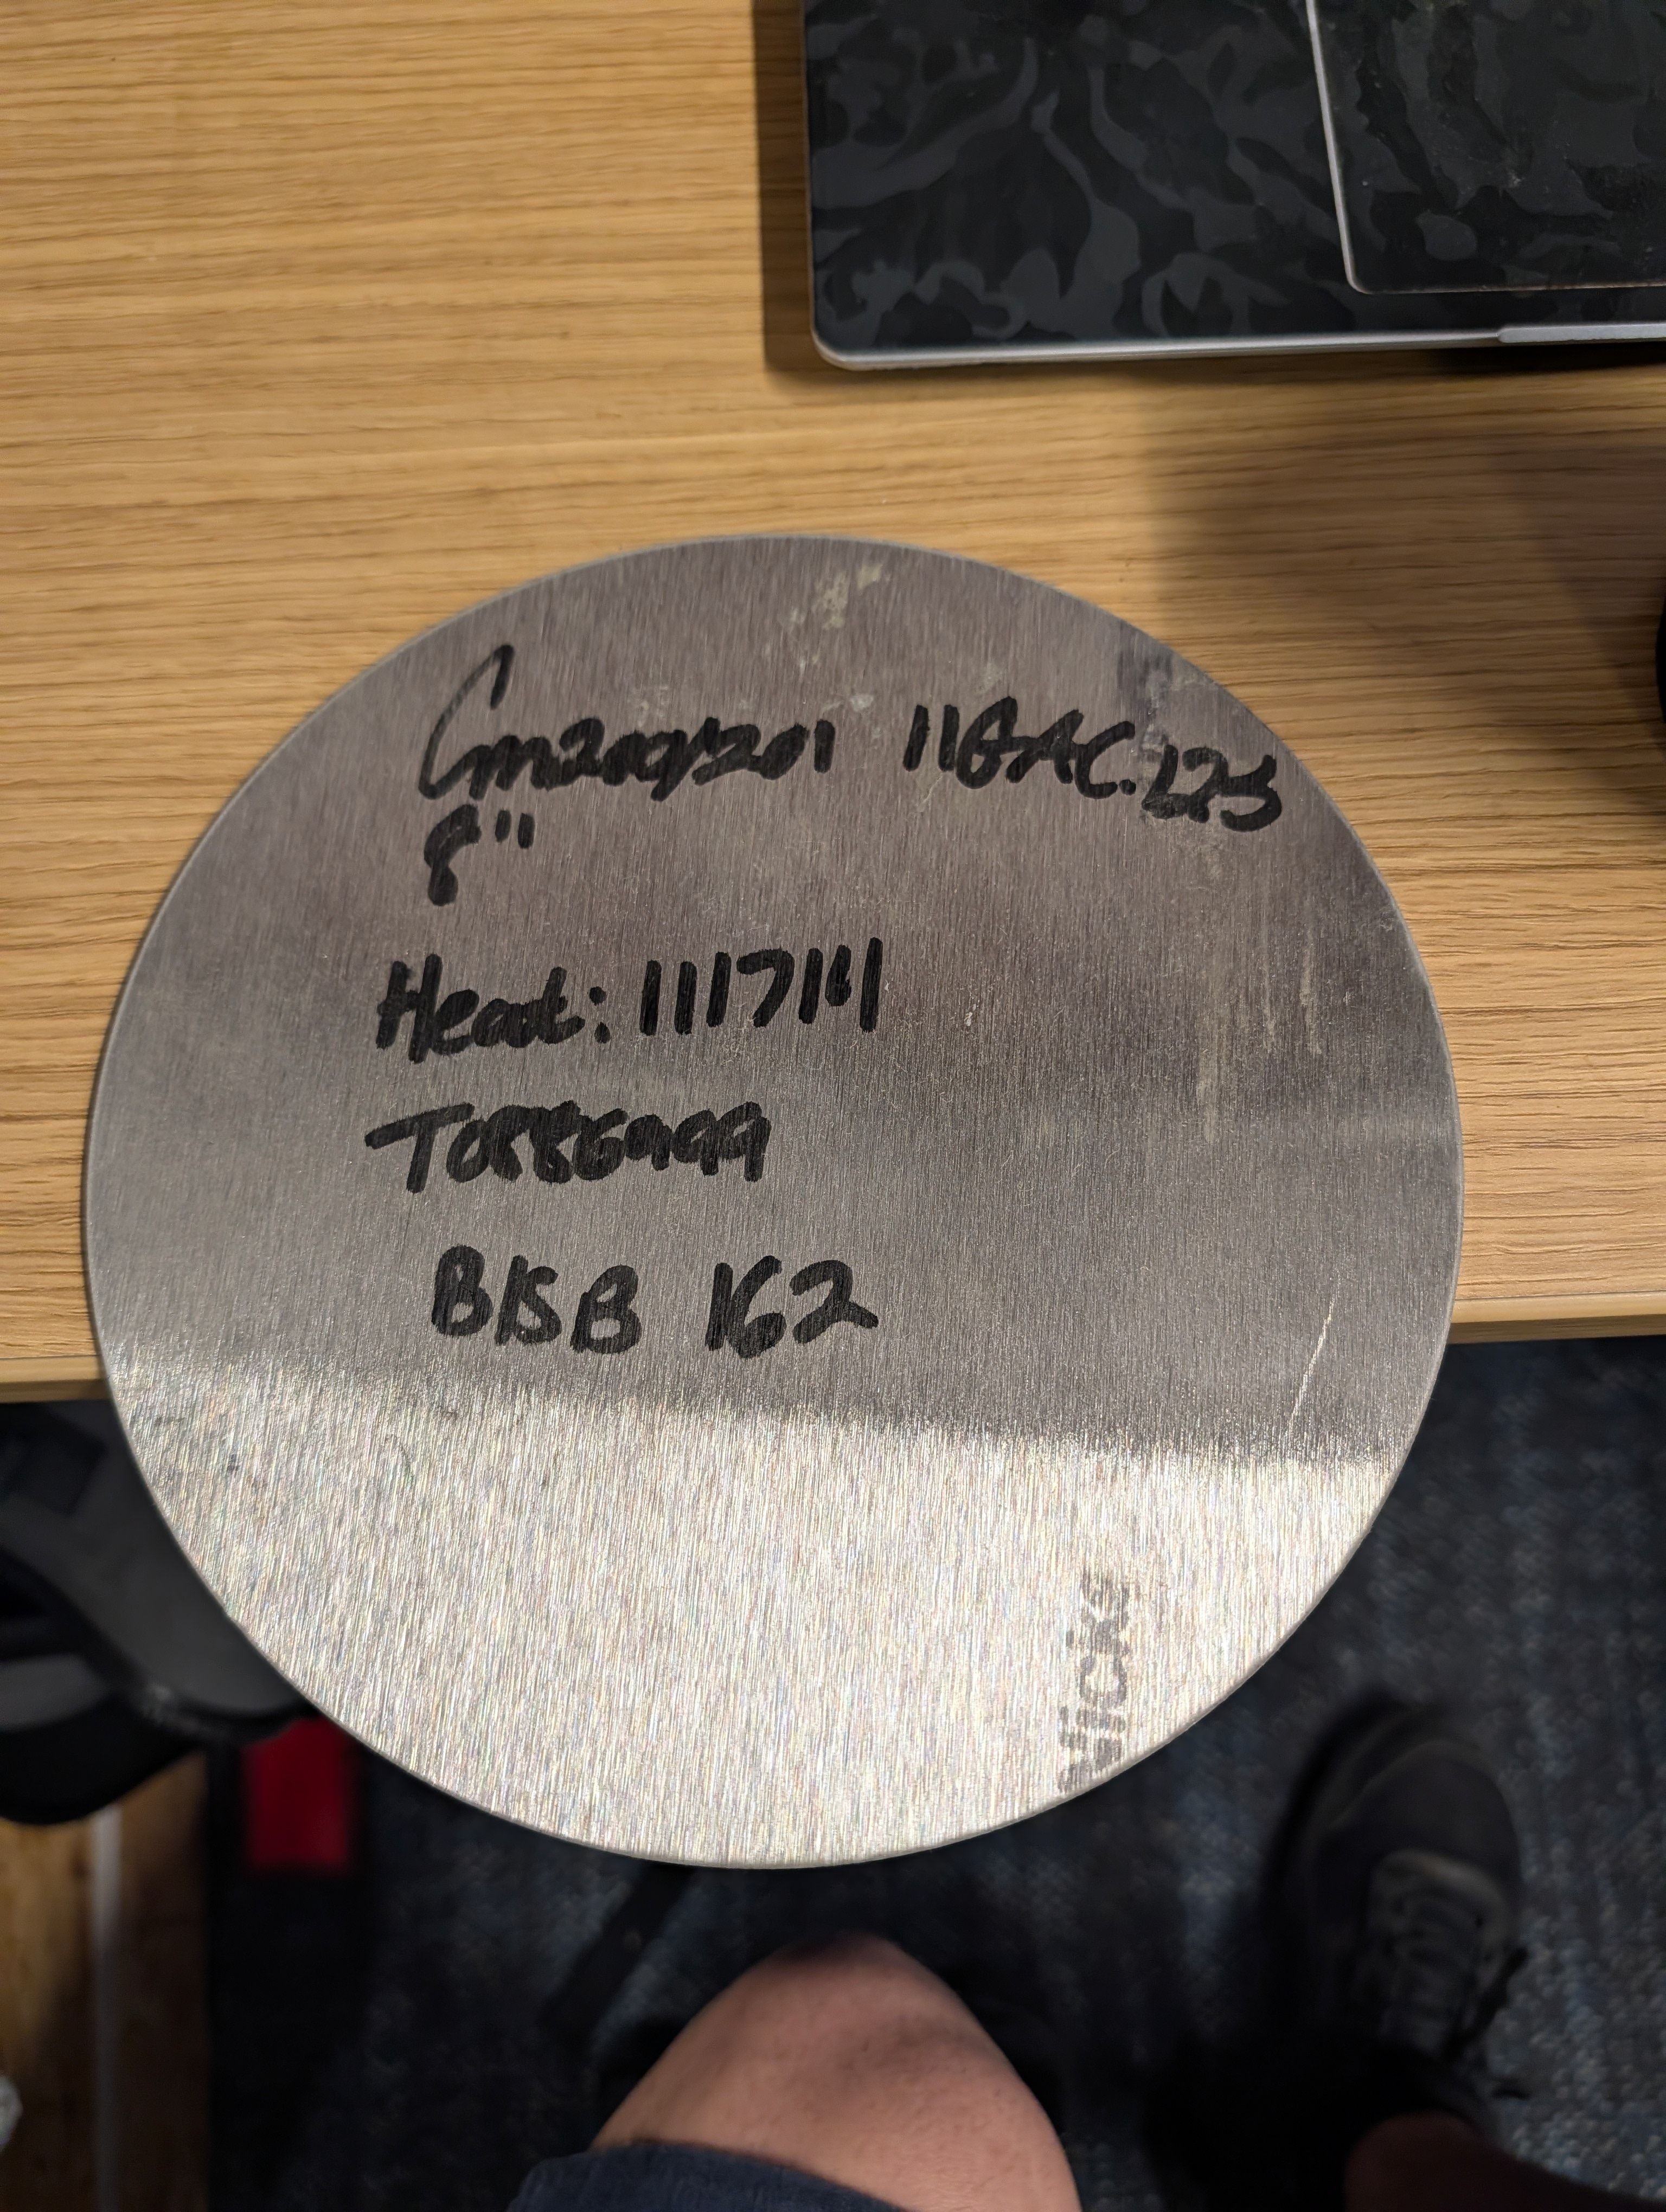
\includegraphics[width=0.6\textwidth]{./assets/pictures/ni round.jpg}
      \caption{Ni round received from Continental}
      \label{fig: liner ni round stock}
    \end{figure}
\end{enumerate}
\pagebreak

Notes on the construction of the Ni liner and welding:
\begin{enumerate}
  \item It was found that the original material purchased for the Ni liner was
    larger than needed. The liner was constructed to be 12" tall and
    an outer diameter of 5.5". % TODO: Note that the excess was
    % recovered, after picking up the material.
  \item A Ni-201 (not confirmed) 1/2" pipe was provided to Brazos
    Industries. They naturally struggled to weld the material.
    A 316L stainless steel tube was provided instead. The weld was
    then quickly completed.
\end{enumerate}
